\section{Anomaliedaten}
\label{sec:data_anomalie}
Um Trainings- und Testdaten für Routen mit Anomalien zu erzeugen, in denen die Sensorbox auf anderen als den üblichen Wegen transportiert wurde,
wurden die bekannten Routen modifiziert, indem Umleitungen eingebaut werden, die teilweise Standorte überspringen und nicht in den Trainingsdaten vorhanden sind.
Dadurch wird ein Szenario simuliert, in der das Klassifizierungsverhalten vom ML-Modell zur Standortbestimmung auf unbekannten Wegen beobachtet werden kann.
Aus den Klassifizierungsergebnissen des ML-Modells zur Standortbestimmung werden schließlich Features extrahiert,
die vom separaten ML-Modell zur Anomalieerkennung verwendet werden.
\begin{figure}[h!]
    \centering
    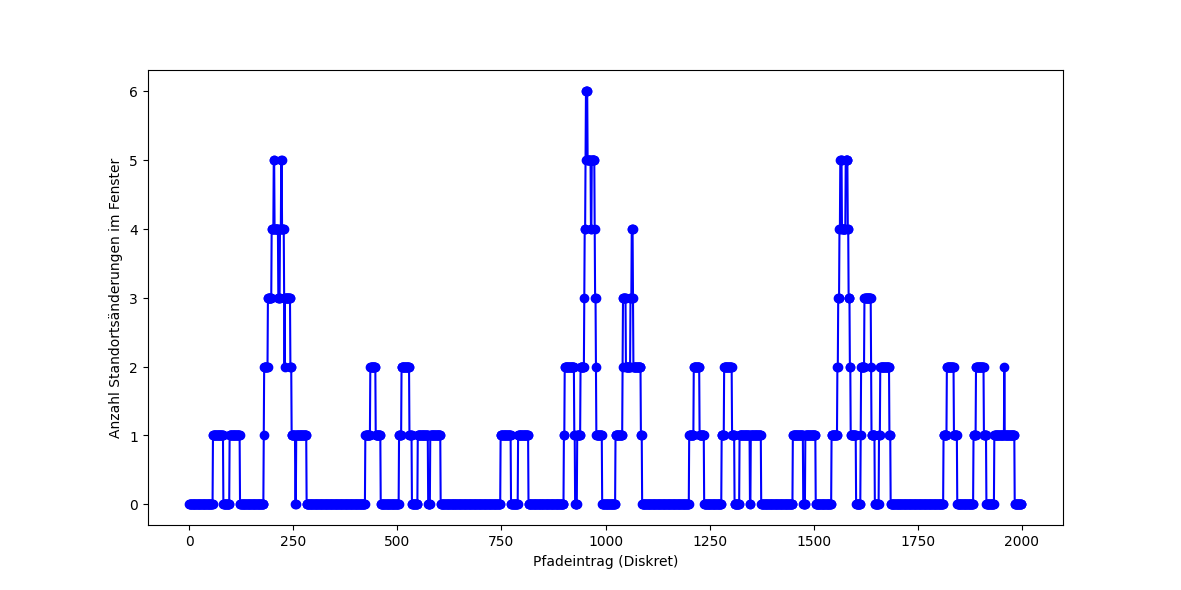
\includegraphics[width=\linewidth]{images/feature_window_location_changes.png}
    \caption{Ausschnitt der Anomalietestmenge mit den Standortänderungen in einem Datenfenster von 25.}
    \label{fig:window_location_changes}
\end{figure}
\newpage
Wenn eine Anomalie vorliegt, wird erwartet, dass das ML-Modell unsicherer wird und stärker fluktuiert,
wodurch drei Features motiviert sind.
Das erste Feature beschreibt die Abweichung von der üblichen Standortänderungshäufigkeit.
Dazu wird der Durchschnitt der aktuellen Häufigkeit der Standortänderungen in einem Datenfenster gemessen und von der durchschnittlichen Häufigkeit ohne Anomalien abgezogen.
Das Feature ist der Betrag dieser Differenz.
Abbildung \ref{fig:window_location_changes} zeigt die akkumulierten Standortänderungen in einem Datenfenster von 25.
Bei den Pfadeinträgen bei ca. 250, 1000 und 1600 sind Extrema zu erkennen, die mit der Anomalie in dieser Testmenge übereinstimmen,
d. h. wenn eine Anomalie vorliegt, wird häufiger der Standort geändert.
\newline
\newline
Das zweite Feature ist analog zum ersten Feature konstruiert.
Dieses nutzt anstatt der Anzahl der Standortänderungen die summierte Wahrscheinlichkeit der erkannten Standorte.
Das ML-Modell zur Standortbestimmung hat keine diskrete Ausgabe, sondern gibt einen Vektor von Wahrscheinlichkeiten aus,
der für jeden Standort die Klassifizierungswahrscheinlichkeit angibt.
Dabei gilt der klassifizierte Standort als der Eintrag im Vektor mit der höchsten Wahrscheinlichkeit.
Diese Wahrscheinlichkeit wird dann analog zu den Standortänderungen akkumuliert.
Das dritte Feature ist die Standardabweichung der ersten fünf Einträge dieses Vektors, der absteigend sortiert ist.
Abbildung \ref{fig:window_confidence} zeigt die akkumulierte Standortwahrscheinlichkeit in einem Datenfenster von 25.
Bei den Pfadeinträgen bei ca. 250, 1000 und 1600 ist die akkumulierte Standortwahrscheinlichkeit deutlich geringer,
d.~h. wenn eine Anomalie vorliegt, ist die Sicherheit für einen Standort geringer.
\begin{figure}[h!]
    \centering
    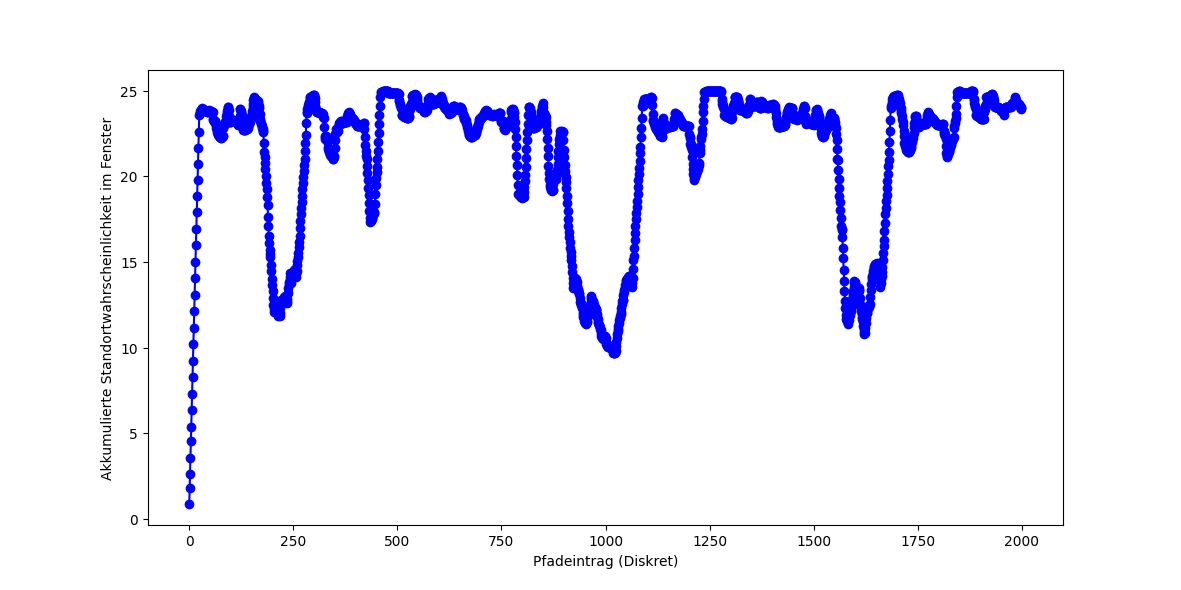
\includegraphics[width=\linewidth]{images/feature_window_confidence.png}
    \caption{Ausschnitt der Anomalietestmenge mit der akkumulierten Standortwahrscheinlichkeit in einem Datenfenster von 25.}
    \label{fig:window_confidence}
\end{figure}
\newline
\newline
Als viertes Feature wird betrachtet, ob die Folge erkannter Standorte einem bekannten Weg entspricht (Listing \ref{lst:topology_anomaly_detection}).
Ist das nicht der Fall, muss das ML-Modell zur Standortbestimmung ein Fehler gemacht haben
oder tatsächlich eine Anomalie vorliegen, da die Topologie verletzt wurde.
\newline
\newline
Daneben wurde ebenfalls eine Rückwärtskante von dem ML-Modell zur Anomalieerkennung zur vorherigen Feature-Extrahierung in Betracht gezogen,
da es wahrscheinlich ist, dass wenn zuvor eine Anomalie vorlag, danach immer noch eine Anomalie vorliegt.
Im Training wurden damit zwar sehr gute Ergebnisse erreicht,
in der Praxis war das Modell aber äquivalent zum \textit{Immer-Falsch}-Modell.
